\section{Morpho-kinematics analysis}

\subsection{$V_{\rm{max}} /\sigma_{\rm{v}}$ distribution}

Medium and high redshift galaxies are classified in kinematics studies as either dispersion dominated or rotationally supported. This can be done if we compute the maximum rotation velocity and the velocity dispersion of our galaxies. The galaxies velocity dispersion is returned as a parameter from the modelling, as well as the curvature radius $R_{\rm{c}}$, the plateau velocity $V_{\rm{c}}$ and the largest radius where the fit was performed $R_{\rm{last}}$. To remain consistent with other studies, we decided to
\begin{enumerate*}[label=(\alph*)]
	\item only keep galaxies with a reliable measure of $V_{\rm{c}}$ such that $R_{\rm{c}} < R_{\rm{last}}$, otherwise the plateau velocity would have to be extrapolated.
	\item compute the maximum rotation velocity of our galaxies at $2.2 R_{\rm{d}}$ with $R_{\rm{d}} \approx 0.5955 R_{1/2}$ the disc scale length (see Appendix \ref{sec:disk_scale_length}.
\end{enumerate*}


\subsection{Tully-Fisher Relation}

\begin{figure}[htbp]
	\centering
	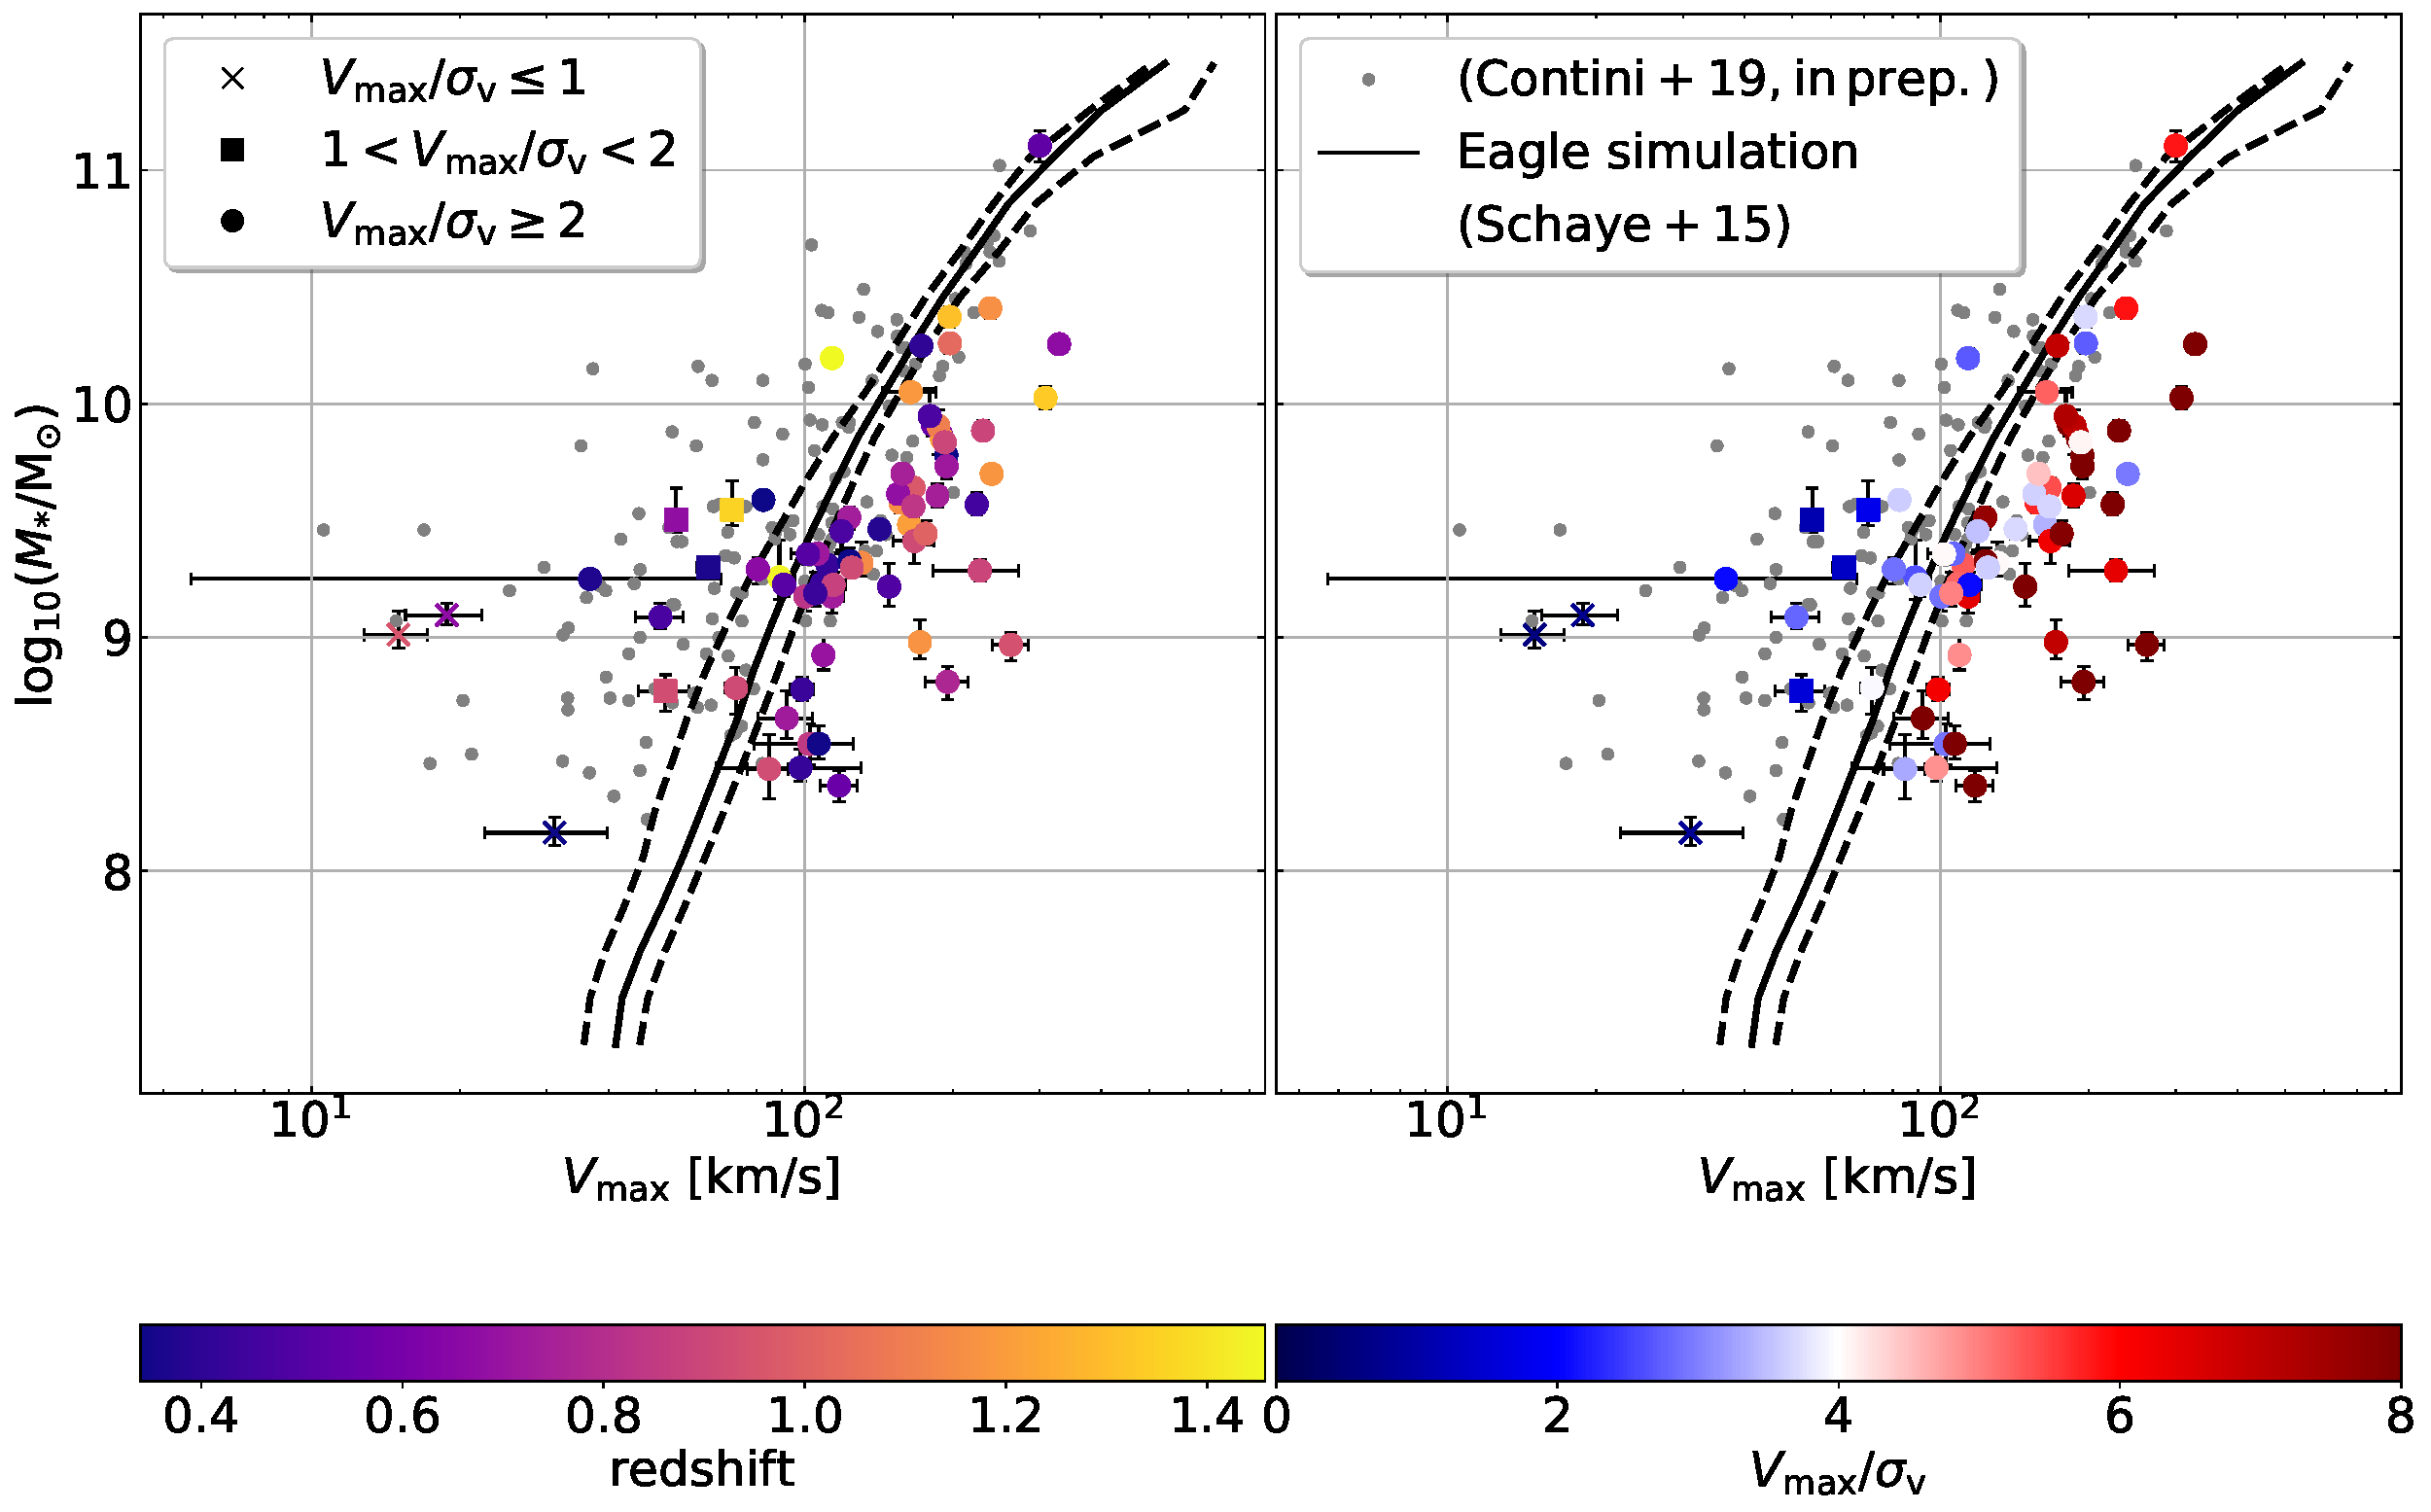
\includegraphics[width=\linewidth]{{../Plots/TFRz}.pdf}
	\caption[Tully-Fisher Relation]{Tully-Fisher Relation
	\begin{enumerate*}[label=]
		\item Left: as a function of redshift.
		\item Right : as a function of $V_{\rm{max}} /\sigma_{\rm{v}}$ ratio.
	\end{enumerate*}		
	In both plots, galaxies have been separated between rotationnaly supported (filled circle), dispersion dominated (cross) and in between (filled square). Error bars correspond to $1\sigma$ uncertainties. The TFR from the Eagle simulation and its errors (plain and dashed lines) are over-plotted for comparison.}
\end{figure}


\newpage
\section{Conclusion}